\documentclass{book}
\usepackage[a4paper,top=2.5cm,bottom=2.5cm,left=2.5cm,right=2.5cm]{geometry}
\usepackage{makeidx}
\usepackage{natbib}
\usepackage{graphicx}
\usepackage{multicol}
\usepackage{float}
\usepackage{listings}
\usepackage{color}
\usepackage{ifthen}
\usepackage[table]{xcolor}
\usepackage{textcomp}
\usepackage{alltt}
\usepackage{ifpdf}
\ifpdf
\usepackage[pdftex,
            pagebackref=true,
            colorlinks=true,
            linkcolor=blue,
            unicode
           ]{hyperref}
\else
\usepackage[ps2pdf,
            pagebackref=true,
            colorlinks=true,
            linkcolor=blue,
            unicode
           ]{hyperref}
\usepackage{pspicture}
\fi
\usepackage[utf8]{inputenc}
\usepackage{mathptmx}
\usepackage[scaled=.90]{helvet}
\usepackage{courier}
\usepackage{sectsty}
\usepackage{amssymb}
\usepackage[titles]{tocloft}
\usepackage{doxygen}
\lstset{language=C++,inputencoding=utf8,basicstyle=\footnotesize,breaklines=true,breakatwhitespace=true,tabsize=4,numbers=left }
\makeindex
\setcounter{tocdepth}{3}
\renewcommand{\footrulewidth}{0.4pt}
\renewcommand{\familydefault}{\sfdefault}
\hfuzz=15pt
\setlength{\emergencystretch}{15pt}
\hbadness=750
\tolerance=750
\begin{document}
\hypersetup{pageanchor=false,citecolor=blue}
\begin{titlepage}
\vspace*{7cm}
\begin{center}
{\Large J\-U\-C\-E Designer }\\
\vspace*{1cm}
{\large Generated by Doxygen 1.8.2-20121118}\\
\vspace*{0.5cm}
{\small Sun Mar 17 2013 04:46:54}\\
\end{center}
\end{titlepage}
\clearemptydoublepage
\pagenumbering{roman}
\tableofcontents
\clearemptydoublepage
\pagenumbering{arabic}
\hypersetup{pageanchor=true,citecolor=blue}
\chapter{Hierarchical Index}
\section{Class Hierarchy}
This inheritance list is sorted roughly, but not completely, alphabetically\-:\begin{DoxyCompactList}
\item \contentsline{section}{Attribute}{\pageref{struct_attribute}}{}
\item Change\-Listener\begin{DoxyCompactList}
\item \contentsline{section}{Colour\-Property\-Component}{\pageref{class_colour_property_component}}{}
\end{DoxyCompactList}
\item Choice\-Property\-Component\begin{DoxyCompactList}
\item \contentsline{section}{Font\-Property\-Component}{\pageref{class_font_property_component}}{}
\end{DoxyCompactList}
\item Component\begin{DoxyCompactList}
\item \contentsline{section}{J\-U\-C\-E\-\_\-\-Designer}{\pageref{class_j_u_c_e___designer}}{}
\item \contentsline{section}{J\-U\-C\-E\-\_\-\-Designer\-:\-:Grid}{\pageref{class_j_u_c_e___designer_1_1_grid}}{}
\item \contentsline{section}{juced\-\_\-\-Main\-Component}{\pageref{classjuced___main_component}}{}
\item \contentsline{section}{Main\-Content\-Component}{\pageref{class_main_content_component}}{}
\item \contentsline{section}{Selection\-Area}{\pageref{class_selection_area}}{}
\item \contentsline{section}{Toolbox}{\pageref{class_toolbox}}{}
\end{DoxyCompactList}
\item \contentsline{section}{Constructor}{\pageref{class_constructor}}{}
\item Deleted\-At\-Shutdown\begin{DoxyCompactList}
\item \contentsline{section}{Font\-List}{\pageref{class_font_list}}{}
\end{DoxyCompactList}
\item Document\-Window\begin{DoxyCompactList}
\item \contentsline{section}{juced\-\_\-\-Window}{\pageref{classjuced___window}}{}
\item \contentsline{section}{juced\-Application\-:\-:Main\-Window}{\pageref{classjuced_application_1_1_main_window}}{}
\end{DoxyCompactList}
\item Dynamic\-Object\begin{DoxyCompactList}
\item \contentsline{section}{juced\-\_\-\-Label}{\pageref{classjuced___label}}{}
\item \contentsline{section}{juced\-\_\-\-Main\-Component}{\pageref{classjuced___main_component}}{}
\item \contentsline{section}{juced\-\_\-\-Text\-Button}{\pageref{classjuced___text_button}}{}
\item \contentsline{section}{juced\-\_\-\-Window}{\pageref{classjuced___window}}{}
\end{DoxyCompactList}
\item J\-U\-C\-E\-Application\begin{DoxyCompactList}
\item \contentsline{section}{juced\-Application}{\pageref{classjuced_application}}{}
\end{DoxyCompactList}
\item Label\begin{DoxyCompactList}
\item \contentsline{section}{juced\-\_\-\-Label}{\pageref{classjuced___label}}{}
\end{DoxyCompactList}
\item Listener\begin{DoxyCompactList}
\item \contentsline{section}{Big\-Tree}{\pageref{class_big_tree}}{}
\end{DoxyCompactList}
\item Listener\begin{DoxyCompactList}
\item \contentsline{section}{Text\-With\-Button\-Property\-Component}{\pageref{class_text_with_button_property_component}}{}
\begin{DoxyCompactList}
\item \contentsline{section}{Colour\-Property\-Component}{\pageref{class_colour_property_component}}{}
\end{DoxyCompactList}
\end{DoxyCompactList}
\item Property\-Panel\begin{DoxyCompactList}
\item \contentsline{section}{Property\-Group}{\pageref{class_property_group}}{}
\end{DoxyCompactList}
\item Text\-Button\begin{DoxyCompactList}
\item \contentsline{section}{juced\-\_\-\-Text\-Button}{\pageref{classjuced___text_button}}{}
\end{DoxyCompactList}
\item Text\-Property\-Component\begin{DoxyCompactList}
\item \contentsline{section}{Text\-With\-Button\-Property\-Component}{\pageref{class_text_with_button_property_component}}{}
\end{DoxyCompactList}
\item Value\-Tree\begin{DoxyCompactList}
\item \contentsline{section}{Big\-Tree}{\pageref{class_big_tree}}{}
\end{DoxyCompactList}
\item Viewport\begin{DoxyCompactList}
\item \contentsline{section}{Property\-View}{\pageref{class_property_view}}{}
\end{DoxyCompactList}
\end{DoxyCompactList}

\chapter{Class Index}
\section{Class List}
Here are the classes, structs, unions and interfaces with brief descriptions\-:\begin{DoxyCompactList}
\item\contentsline{section}{\hyperlink{struct_attribute}{Attribute} \\*Struct to hold all parameters of a given attribute identifier }{\pageref{struct_attribute}}{}
\item\contentsline{section}{\hyperlink{class_big_tree}{Big\-Tree} }{\pageref{class_big_tree}}{}
\item\contentsline{section}{\hyperlink{class_colour_property_component}{Colour\-Property\-Component} }{\pageref{class_colour_property_component}}{}
\item\contentsline{section}{\hyperlink{class_constructor}{Constructor} \\*Object required to build components and show its properties }{\pageref{class_constructor}}{}
\item\contentsline{section}{\hyperlink{class_font_list}{Font\-List} }{\pageref{class_font_list}}{}
\item\contentsline{section}{\hyperlink{class_font_property_component}{Font\-Property\-Component} }{\pageref{class_font_property_component}}{}
\item\contentsline{section}{\hyperlink{class_j_u_c_e___designer_1_1_grid}{J\-U\-C\-E\-\_\-\-Designer\-::\-Grid} }{\pageref{class_j_u_c_e___designer_1_1_grid}}{}
\item\contentsline{section}{\hyperlink{class_j_u_c_e___designer}{J\-U\-C\-E\-\_\-\-Designer} }{\pageref{class_j_u_c_e___designer}}{}
\item\contentsline{section}{\hyperlink{classjuced___label}{juced\-\_\-\-Label} }{\pageref{classjuced___label}}{}
\item\contentsline{section}{\hyperlink{classjuced___main_component}{juced\-\_\-\-Main\-Component} }{\pageref{classjuced___main_component}}{}
\item\contentsline{section}{\hyperlink{classjuced___text_button}{juced\-\_\-\-Text\-Button} }{\pageref{classjuced___text_button}}{}
\item\contentsline{section}{\hyperlink{classjuced___window}{juced\-\_\-\-Window} }{\pageref{classjuced___window}}{}
\item\contentsline{section}{\hyperlink{classjuced_application}{juced\-Application} }{\pageref{classjuced_application}}{}
\item\contentsline{section}{\hyperlink{class_main_content_component}{Main\-Content\-Component} }{\pageref{class_main_content_component}}{}
\item\contentsline{section}{\hyperlink{classjuced_application_1_1_main_window}{juced\-Application\-::\-Main\-Window} }{\pageref{classjuced_application_1_1_main_window}}{}
\item\contentsline{section}{\hyperlink{class_property_group}{Property\-Group} }{\pageref{class_property_group}}{}
\item\contentsline{section}{\hyperlink{class_property_view}{Property\-View} }{\pageref{class_property_view}}{}
\item\contentsline{section}{\hyperlink{class_selection_area}{Selection\-Area} }{\pageref{class_selection_area}}{}
\item\contentsline{section}{\hyperlink{class_text_with_button_property_component}{Text\-With\-Button\-Property\-Component} }{\pageref{class_text_with_button_property_component}}{}
\item\contentsline{section}{\hyperlink{class_toolbox}{Toolbox} }{\pageref{class_toolbox}}{}
\end{DoxyCompactList}

\chapter{Class Documentation}
\hypertarget{struct_attribute}{\section{Attribute Struct Reference}
\label{struct_attribute}\index{Attribute@{Attribute}}
}


Struct to hold all parameters of a given attribute identifier.  




{\ttfamily \#include $<$Constructor.\-h$>$}

\subsection*{Public Attributes}
\begin{DoxyCompactItemize}
\item 
\hypertarget{struct_attribute_a365b41cf28a792401ad145529e8e0980}{Identifier {\bfseries name}}\label{struct_attribute_a365b41cf28a792401ad145529e8e0980}

\item 
\hypertarget{struct_attribute_a507acf1e4de2cd6da2a6ddb116b2a90f}{String {\bfseries group}}\label{struct_attribute_a507acf1e4de2cd6da2a6ddb116b2a90f}

\item 
\hypertarget{struct_attribute_a83dafc8acd95332429cc74120d847b44}{bool {\bfseries visible}}\label{struct_attribute_a83dafc8acd95332429cc74120d847b44}

\item 
\hypertarget{struct_attribute_a4c8a15a28e43ae4395feec8ce19c32aa}{Identifier {\bfseries type}}\label{struct_attribute_a4c8a15a28e43ae4395feec8ce19c32aa}

\item 
\hypertarget{struct_attribute_a1fcda51258d72e64a8c2527bd723c2fa}{String {\bfseries display}}\label{struct_attribute_a1fcda51258d72e64a8c2527bd723c2fa}

\item 
\hypertarget{struct_attribute_a6b736c33181fe639b8fd9339c36c1f1e}{Identifier {\bfseries value\-Type}}\label{struct_attribute_a6b736c33181fe639b8fd9339c36c1f1e}

\end{DoxyCompactItemize}


\subsection{Detailed Description}
Struct to hold all parameters of a given attribute identifier. 

\begin{DoxySeeAlso}{See Also}
get\-Attribute\-Of 

Attributes 
\end{DoxySeeAlso}


The documentation for this struct was generated from the following file\-:\begin{DoxyCompactItemize}
\item 
Designer/Constructor.\-h\end{DoxyCompactItemize}

\hypertarget{class_big_tree}{\section{Big\-Tree Class Reference}
\label{class_big_tree}\index{Big\-Tree@{Big\-Tree}}
}
Inheritance diagram for Big\-Tree\-:\begin{figure}[H]
\begin{center}
\leavevmode
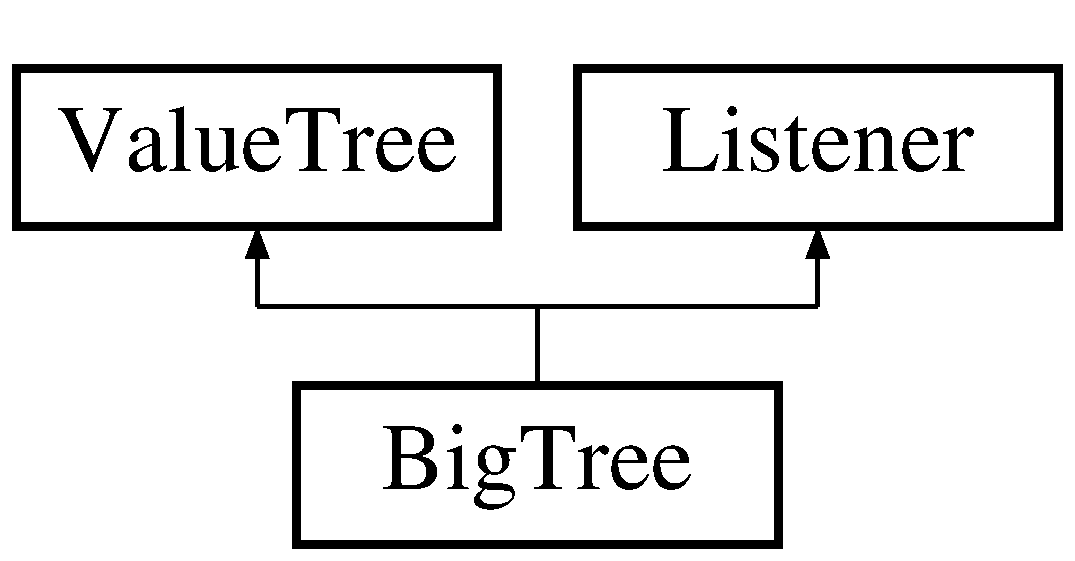
\includegraphics[height=2.000000cm]{class_big_tree}
\end{center}
\end{figure}
\subsection*{Public Member Functions}
\begin{DoxyCompactItemize}
\item 
\hypertarget{class_big_tree_a673a227c948d0a7fef8adacebdd6295b}{{\bfseries Big\-Tree} (const Value\-Tree \&other)}\label{class_big_tree_a673a227c948d0a7fef8adacebdd6295b}

\item 
\hypertarget{class_big_tree_acd2251e281a39ccefb6056450384abab}{{\bfseries Big\-Tree} (Dynamic\-Object $\ast$object, var \-\_\-type)}\label{class_big_tree_acd2251e281a39ccefb6056450384abab}

\item 
\hypertarget{class_big_tree_a4084e1b33ee27cddda808349c85aa351}{{\bfseries Big\-Tree} (Dynamic\-Object $\ast$object)}\label{class_big_tree_a4084e1b33ee27cddda808349c85aa351}

\item 
\hypertarget{class_big_tree_a6e08df0b0f2f20f1feedd3bad154c4c4}{void {\bfseries value\-Tree\-Property\-Changed} (Value\-Tree \&tree\-Whose\-Property\-Has\-Changed, const Identifier \&property)}\label{class_big_tree_a6e08df0b0f2f20f1feedd3bad154c4c4}

\item 
\hypertarget{class_big_tree_acc87d5d7c4737291733c5b8d2e5b02d4}{void {\bfseries value\-Tree\-Child\-Added} (Value\-Tree \&parent\-Tree, Value\-Tree \&child\-Which\-Has\-Been\-Added)}\label{class_big_tree_acc87d5d7c4737291733c5b8d2e5b02d4}

\item 
\hypertarget{class_big_tree_ae82fe163ef2366682c39fb54e42d952a}{void {\bfseries value\-Tree\-Child\-Removed} (Value\-Tree \&parent\-Tree, Value\-Tree \&child\-Which\-Has\-Been\-Removed)}\label{class_big_tree_ae82fe163ef2366682c39fb54e42d952a}

\item 
\hypertarget{class_big_tree_a062315a1f47244573a8c68555fa61e26}{void {\bfseries value\-Tree\-Child\-Order\-Changed} (Value\-Tree \&parent\-Tree\-Whose\-Children\-Have\-Moved)}\label{class_big_tree_a062315a1f47244573a8c68555fa61e26}

\item 
\hypertarget{class_big_tree_a80330adcc8f2a0f1f64a1eec8c73a2f3}{void {\bfseries value\-Tree\-Parent\-Changed} (Value\-Tree \&tree\-Whose\-Parent\-Has\-Changed)}\label{class_big_tree_a80330adcc8f2a0f1f64a1eec8c73a2f3}

\item 
\hypertarget{class_big_tree_ad51b3c047e9d1106943193818825a288}{void {\bfseries value\-Tree\-Redirected} (Value\-Tree \&tree\-Which\-Has\-Been\-Changed)}\label{class_big_tree_ad51b3c047e9d1106943193818825a288}

\item 
\hypertarget{class_big_tree_a2e9da63624e0c7982e12aab3f1361f32}{\hyperlink{class_big_tree}{Big\-Tree} \& {\bfseries get\-Child\-With\-Property} (const Identifier \&property\-Name, const var \&property\-Value, bool recursive)}\label{class_big_tree_a2e9da63624e0c7982e12aab3f1361f32}

\item 
\hypertarget{class_big_tree_ac2c384997bb5faf0d18e6852c3eb2941}{\hyperlink{class_big_tree}{Big\-Tree} {\bfseries get\-Child} (int index) const }\label{class_big_tree_ac2c384997bb5faf0d18e6852c3eb2941}

\item 
\hypertarget{class_big_tree_a47a9f19b49792e570174ff0773ba1d78}{void {\bfseries recursive\-\_\-remove\-Property} (Identifier name, Undo\-Manager $\ast$undo\-Manager)}\label{class_big_tree_a47a9f19b49792e570174ff0773ba1d78}

\item 
\hypertarget{class_big_tree_af7fff16ebcf45fe76905e025e25f5442}{Xml\-Element $\ast$ {\bfseries create\-Xml} ()}\label{class_big_tree_af7fff16ebcf45fe76905e025e25f5442}

\end{DoxyCompactItemize}


The documentation for this class was generated from the following file\-:\begin{DoxyCompactItemize}
\item 
Designer/Big\-Tree.\-cpp\end{DoxyCompactItemize}

\hypertarget{class_colour_property_component}{\section{Colour\-Property\-Component Class Reference}
\label{class_colour_property_component}\index{Colour\-Property\-Component@{Colour\-Property\-Component}}
}
Inheritance diagram for Colour\-Property\-Component\-:\begin{figure}[H]
\begin{center}
\leavevmode
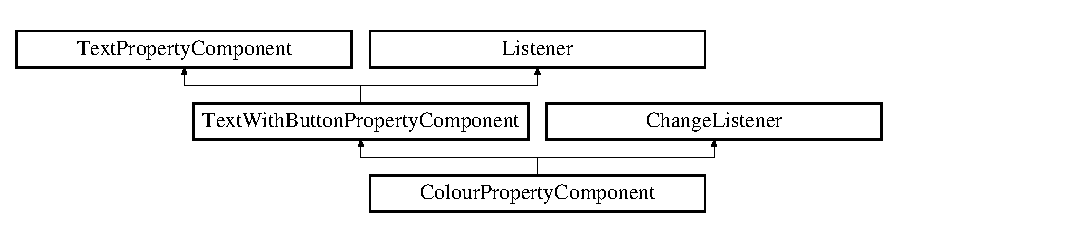
\includegraphics[height=2.616822cm]{class_colour_property_component}
\end{center}
\end{figure}
\subsection*{Public Member Functions}
\begin{DoxyCompactItemize}
\item 
\hypertarget{class_colour_property_component_a66a36b844a4615df46ee22ef23312dd3}{{\bfseries Colour\-Property\-Component} (const Value \&Value\-To\-Control, const String \&property\-Name)}\label{class_colour_property_component_a66a36b844a4615df46ee22ef23312dd3}

\item 
\hypertarget{class_colour_property_component_ac4cba912636746ed27d69873f4699855}{void {\bfseries button\-Clicked} (Button $\ast$button\-That\-Was\-Clicked)}\label{class_colour_property_component_ac4cba912636746ed27d69873f4699855}

\item 
\hypertarget{class_colour_property_component_a6799c4e985e7907485d3e45721d1011c}{void {\bfseries change\-Listener\-Callback} (Change\-Broadcaster $\ast$source)}\label{class_colour_property_component_a6799c4e985e7907485d3e45721d1011c}

\end{DoxyCompactItemize}
\subsection*{Public Attributes}
\begin{DoxyCompactItemize}
\item 
\hypertarget{class_colour_property_component_a3420be208116eb02d4a9c9d661249a00}{Colour {\bfseries colour}}\label{class_colour_property_component_a3420be208116eb02d4a9c9d661249a00}

\end{DoxyCompactItemize}


The documentation for this class was generated from the following file\-:\begin{DoxyCompactItemize}
\item 
Designer/Properties\-Component.\-cpp\end{DoxyCompactItemize}

\hypertarget{class_constructor}{\section{Constructor Class Reference}
\label{class_constructor}\index{Constructor@{Constructor}}
}


Object required to build components and show its properties.  




{\ttfamily \#include $<$Constructor.\-h$>$}

\subsection*{Public Member Functions}
\begin{DoxyCompactItemize}
\item 
void \hyperlink{class_constructor_aa276e1e035578f7964780a2f3453395f}{load\-Attributes\-From\-Xml\-File} (const File \&xml\-File)
\begin{DoxyCompactList}\small\item\em Function called within \hyperlink{class_j_u_c_e___designer}{J\-U\-C\-E\-\_\-\-Designer} constructor. \end{DoxyCompactList}\item 
\hyperlink{struct_attribute}{Attribute} $\ast$ \hyperlink{class_constructor_ab34f1e9062445681a508550415ff18ef}{get\-Attribute\-Of} (Identifier \-\_\-name)
\begin{DoxyCompactList}\small\item\em Returns a struct pointer of attribute parameters given it's Identifier. \end{DoxyCompactList}\end{DoxyCompactItemize}
\subsection*{Static Public Member Functions}
\begin{DoxyCompactItemize}
\item 
static \hyperlink{class_constructor}{Constructor} $\ast$ \hyperlink{class_constructor_a757cc1671f52f15291b89772bef7aa98}{get\-Instance} ()
\begin{DoxyCompactList}\small\item\em This function is called to create an instance of the class. \end{DoxyCompactList}\end{DoxyCompactItemize}
\subsection*{Public Attributes}
\begin{DoxyCompactItemize}
\item 
\hypertarget{class_constructor_ae5d823f5aaef582e23842ee45a001c12}{Array$<$ \hyperlink{struct_attribute}{Attribute} $\ast$ $>$ {\bfseries \-\_\-attributes}}\label{class_constructor_ae5d823f5aaef582e23842ee45a001c12}

\end{DoxyCompactItemize}


\subsection{Detailed Description}
Object required to build components and show its properties. 

Only one instance of this object is allowed.

To use, simply get an instance of this class using the \hyperlink{class_constructor_a757cc1671f52f15291b89772bef7aa98}{get\-Instance()} static method. Example\-: \hyperlink{class_constructor}{Constructor} $\ast$constructor = \hyperlink{class_constructor_a757cc1671f52f15291b89772bef7aa98}{Constructor\-::get\-Instance()}; 

\subsection{Member Function Documentation}
\hypertarget{class_constructor_ab34f1e9062445681a508550415ff18ef}{\index{Constructor@{Constructor}!get\-Attribute\-Of@{get\-Attribute\-Of}}
\index{get\-Attribute\-Of@{get\-Attribute\-Of}!Constructor@{Constructor}}
\subsubsection[{get\-Attribute\-Of}]{\setlength{\rightskip}{0pt plus 5cm}{\bf Attribute} $\ast$ Constructor\-::get\-Attribute\-Of (
\begin{DoxyParamCaption}
\item[{Identifier}]{\-\_\-name}
\end{DoxyParamCaption}
)}}\label{class_constructor_ab34f1e9062445681a508550415ff18ef}


Returns a struct pointer of attribute parameters given it's Identifier. 


\begin{DoxyParams}{Parameters}
{\em \-\_\-name} & \hyperlink{struct_attribute}{Attribute} identifier. \\
\hline
\end{DoxyParams}
\begin{DoxySeeAlso}{See Also}
\hyperlink{struct_attribute}{Attribute} 

Attributes 
\end{DoxySeeAlso}
\hypertarget{class_constructor_a757cc1671f52f15291b89772bef7aa98}{\index{Constructor@{Constructor}!get\-Instance@{get\-Instance}}
\index{get\-Instance@{get\-Instance}!Constructor@{Constructor}}
\subsubsection[{get\-Instance}]{\setlength{\rightskip}{0pt plus 5cm}{\bf Constructor} $\ast$ Constructor\-::get\-Instance (
\begin{DoxyParamCaption}
{}
\end{DoxyParamCaption}
)\hspace{0.3cm}{\ttfamily [static]}}}\label{class_constructor_a757cc1671f52f15291b89772bef7aa98}


This function is called to create an instance of the class. 

Calling the constructor publicly is not allowed. The constructor is private and is only called by this Instance function. \hypertarget{class_constructor_aa276e1e035578f7964780a2f3453395f}{\index{Constructor@{Constructor}!load\-Attributes\-From\-Xml\-File@{load\-Attributes\-From\-Xml\-File}}
\index{load\-Attributes\-From\-Xml\-File@{load\-Attributes\-From\-Xml\-File}!Constructor@{Constructor}}
\subsubsection[{load\-Attributes\-From\-Xml\-File}]{\setlength{\rightskip}{0pt plus 5cm}void Constructor\-::load\-Attributes\-From\-Xml\-File (
\begin{DoxyParamCaption}
\item[{const File \&}]{xml\-File}
\end{DoxyParamCaption}
)}}\label{class_constructor_aa276e1e035578f7964780a2f3453395f}


Function called within \hyperlink{class_j_u_c_e___designer}{J\-U\-C\-E\-\_\-\-Designer} constructor. 

Loads all parameters from a list of attribute types in a X\-M\-L file.


\begin{DoxyParams}{Parameters}
{\em xml\-File} & File object that points to X\-M\-L file in disc. \\
\hline
\end{DoxyParams}
\begin{DoxySeeAlso}{See Also}
\hyperlink{class_constructor_ab34f1e9062445681a508550415ff18ef}{get\-Attribute\-Of} 
\end{DoxySeeAlso}


The documentation for this class was generated from the following files\-:\begin{DoxyCompactItemize}
\item 
Designer/Constructor.\-h\item 
Designer/Constructor.\-cpp\end{DoxyCompactItemize}

\hypertarget{class_font_list}{\section{Font\-List Class Reference}
\label{class_font_list}\index{Font\-List@{Font\-List}}
}
Inheritance diagram for Font\-List\-:\begin{figure}[H]
\begin{center}
\leavevmode
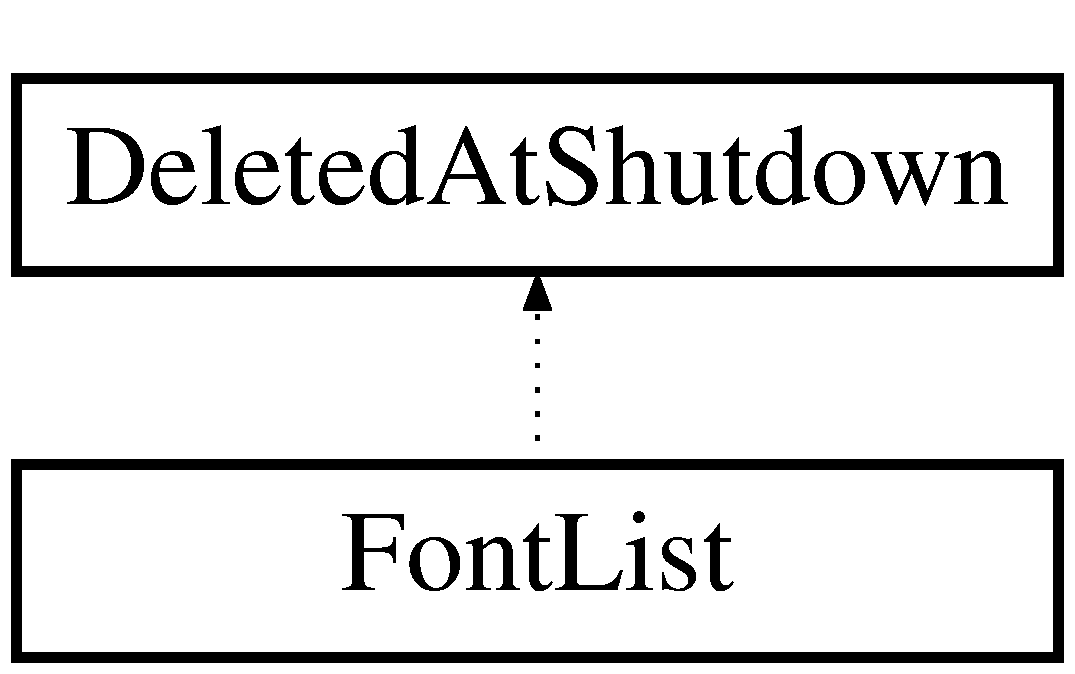
\includegraphics[height=2.000000cm]{class_font_list}
\end{center}
\end{figure}
\subsection*{Public Member Functions}
\begin{DoxyCompactItemize}
\item 
\hypertarget{class_font_list_ae59193ebb75a13ceef77324e1a06e13d}{{\bfseries juce\-\_\-\-Declare\-Singleton\-\_\-\-Single\-Threaded\-\_\-\-Minimal} (\hyperlink{class_font_list}{Font\-List}) String\-Array font\-Names}\label{class_font_list_ae59193ebb75a13ceef77324e1a06e13d}

\end{DoxyCompactItemize}


The documentation for this class was generated from the following file\-:\begin{DoxyCompactItemize}
\item 
Designer/\-Properties/Font\-Property\-Component.\-cpp\end{DoxyCompactItemize}

\hypertarget{class_font_property_component}{\section{Font\-Property\-Component Class Reference}
\label{class_font_property_component}\index{Font\-Property\-Component@{Font\-Property\-Component}}
}
Inheritance diagram for Font\-Property\-Component\-:\begin{figure}[H]
\begin{center}
\leavevmode
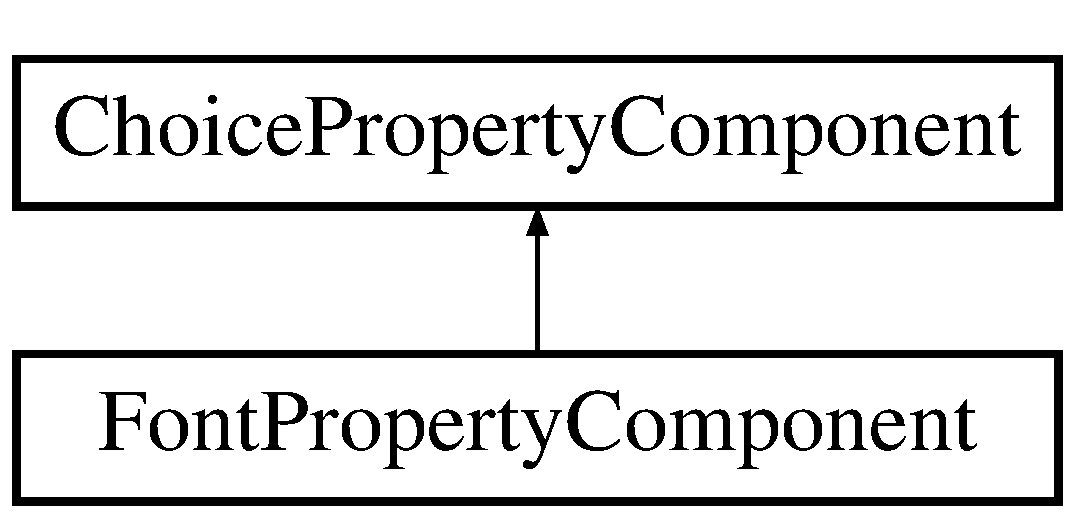
\includegraphics[height=2.000000cm]{class_font_property_component}
\end{center}
\end{figure}
\subsection*{Public Member Functions}
\begin{DoxyCompactItemize}
\item 
\hypertarget{class_font_property_component_a47de1b91d7384af600c0c9cb4e41ca03}{{\bfseries Font\-Property\-Component} (const String \&name)}\label{class_font_property_component_a47de1b91d7384af600c0c9cb4e41ca03}

\item 
\hypertarget{class_font_property_component_a31e0cf1899d88abecfa989559dafa9f1}{virtual void {\bfseries set\-Typeface\-Name} (const String \&new\-Font\-Name)=0}\label{class_font_property_component_a31e0cf1899d88abecfa989559dafa9f1}

\item 
\hypertarget{class_font_property_component_a8de426b0fef660d4e028fc77e8d4ae08}{virtual String {\bfseries get\-Typeface\-Name} () const =0}\label{class_font_property_component_a8de426b0fef660d4e028fc77e8d4ae08}

\item 
\hypertarget{class_font_property_component_ab9d8f5b104b1702b1e38cf70af7ade9b}{void {\bfseries set\-Index} (int new\-Index)}\label{class_font_property_component_ab9d8f5b104b1702b1e38cf70af7ade9b}

\item 
\hypertarget{class_font_property_component_a395aacef9bf0ab9911c061a1f21d0887}{int {\bfseries get\-Index} () const }\label{class_font_property_component_a395aacef9bf0ab9911c061a1f21d0887}

\end{DoxyCompactItemize}
\subsection*{Static Public Member Functions}
\begin{DoxyCompactItemize}
\item 
\hypertarget{class_font_property_component_a433c79a35b89d5c333e39219bec49afe}{static void {\bfseries preload\-All\-Fonts} ()}\label{class_font_property_component_a433c79a35b89d5c333e39219bec49afe}

\item 
\hypertarget{class_font_property_component_a22427cbec8c6b15fa3ee586fdcfcb113}{static const Font {\bfseries apply\-Name\-To\-Font} (const String \&typeface\-Name, const Font \&font)}\label{class_font_property_component_a22427cbec8c6b15fa3ee586fdcfcb113}

\item 
\hypertarget{class_font_property_component_ad2f0ebaab2d6c0d736541ef30a062f51}{static const String {\bfseries get\-Typeface\-Name\-Code} (const String \&typeface\-Name)}\label{class_font_property_component_ad2f0ebaab2d6c0d736541ef30a062f51}

\item 
\hypertarget{class_font_property_component_aefaf8dd5558151e98958edb83a0b57c2}{static const String {\bfseries get\-Font\-Style\-Code} (const Font \&font)}\label{class_font_property_component_aefaf8dd5558151e98958edb83a0b57c2}

\item 
\hypertarget{class_font_property_component_a2f77cd1095c970f5497026d28f1656a4}{static const String {\bfseries get\-Complete\-Font\-Code} (const Font \&font, const String \&typeface\-Name)}\label{class_font_property_component_a2f77cd1095c970f5497026d28f1656a4}

\end{DoxyCompactItemize}
\subsection*{Static Public Attributes}
\begin{DoxyCompactItemize}
\item 
\hypertarget{class_font_property_component_a70b8b855124183179d76caf5c60e8377}{static const String {\bfseries default\-Font}}\label{class_font_property_component_a70b8b855124183179d76caf5c60e8377}

\item 
\hypertarget{class_font_property_component_a3279e79714cbf392f9851fab5d49a5f4}{static const String {\bfseries default\-Sans}}\label{class_font_property_component_a3279e79714cbf392f9851fab5d49a5f4}

\item 
\hypertarget{class_font_property_component_a334be8c1959ab0c870c1378ff1cea4b7}{static const String {\bfseries default\-Serif}}\label{class_font_property_component_a334be8c1959ab0c870c1378ff1cea4b7}

\item 
\hypertarget{class_font_property_component_a939f3dad9a05faf4e12169679a7faefa}{static const String {\bfseries default\-Mono}}\label{class_font_property_component_a939f3dad9a05faf4e12169679a7faefa}

\end{DoxyCompactItemize}


The documentation for this class was generated from the following files\-:\begin{DoxyCompactItemize}
\item 
Designer/\-Properties/Font\-Property\-Component.\-h\item 
Designer/\-Properties/Font\-Property\-Component.\-cpp\end{DoxyCompactItemize}

\hypertarget{class_j_u_c_e___designer_1_1_grid}{\section{J\-U\-C\-E\-\_\-\-Designer\-:\-:Grid Class Reference}
\label{class_j_u_c_e___designer_1_1_grid}\index{J\-U\-C\-E\-\_\-\-Designer\-::\-Grid@{J\-U\-C\-E\-\_\-\-Designer\-::\-Grid}}
}
Inheritance diagram for J\-U\-C\-E\-\_\-\-Designer\-:\-:Grid\-:\begin{figure}[H]
\begin{center}
\leavevmode
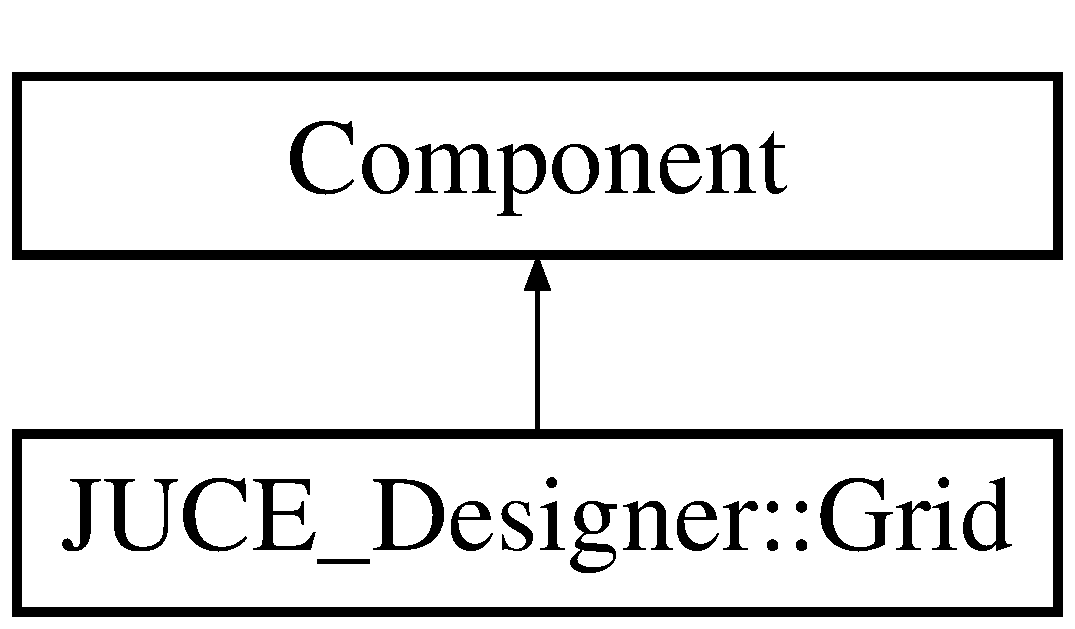
\includegraphics[height=2.000000cm]{class_j_u_c_e___designer_1_1_grid}
\end{center}
\end{figure}
\subsection*{Public Member Functions}
\begin{DoxyCompactItemize}
\item 
\hypertarget{class_j_u_c_e___designer_1_1_grid_a2cb60e91219a599c0b03f72fc0be37c5}{void {\bfseries paint} (Graphics \&g)}\label{class_j_u_c_e___designer_1_1_grid_a2cb60e91219a599c0b03f72fc0be37c5}

\end{DoxyCompactItemize}


The documentation for this class was generated from the following files\-:\begin{DoxyCompactItemize}
\item 
J\-U\-C\-E\-\_\-\-Designer.\-h\item 
J\-U\-C\-E\-\_\-\-Designer.\-cpp\end{DoxyCompactItemize}

\hypertarget{class_j_u_c_e___designer}{\section{J\-U\-C\-E\-\_\-\-Designer Class Reference}
\label{class_j_u_c_e___designer}\index{J\-U\-C\-E\-\_\-\-Designer@{J\-U\-C\-E\-\_\-\-Designer}}
}
Inheritance diagram for J\-U\-C\-E\-\_\-\-Designer\-:\begin{figure}[H]
\begin{center}
\leavevmode
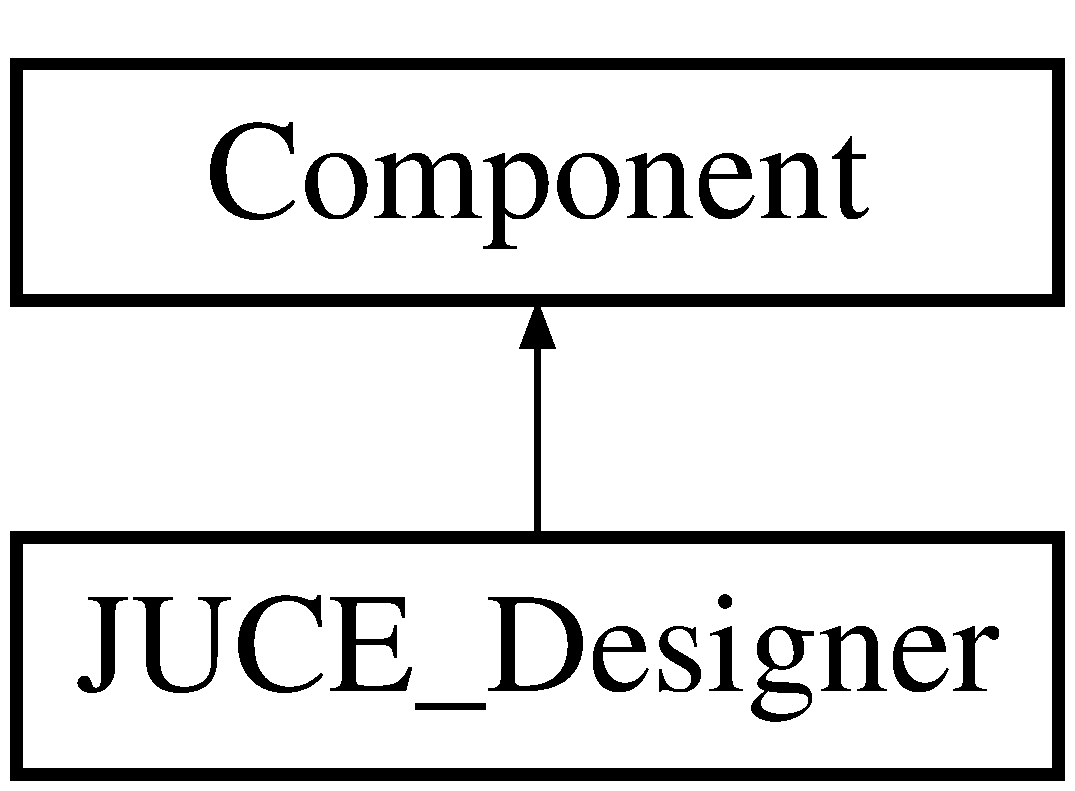
\includegraphics[height=2.000000cm]{class_j_u_c_e___designer}
\end{center}
\end{figure}
\subsection*{Classes}
\begin{DoxyCompactItemize}
\item 
class \hyperlink{class_j_u_c_e___designer_1_1_grid}{Grid}
\end{DoxyCompactItemize}
\subsection*{Public Member Functions}
\begin{DoxyCompactItemize}
\item 
\hypertarget{class_j_u_c_e___designer_a99543579daf52cfa413726bb360d2149}{Component $\ast$ {\bfseries create\-Toolbox} (int items\-Per\-Row, int item\-Size, int item\-Padding)}\label{class_j_u_c_e___designer_a99543579daf52cfa413726bb360d2149}

\item 
\hypertarget{class_j_u_c_e___designer_afc5109b1e779cab9a2c1dcab7a041dd0}{void {\bfseries add\-Toolbox\-Item} (Component $\ast$toolbox, const String \&name, const String \&tool\-Tip, const char $\ast$image, int image\-Size)}\label{class_j_u_c_e___designer_afc5109b1e779cab9a2c1dcab7a041dd0}

\item 
\hypertarget{class_j_u_c_e___designer_a017758c079bd2aa84023d5a60e892fd4}{Viewport $\ast$ {\bfseries get\-Property\-View} ()}\label{class_j_u_c_e___designer_a017758c079bd2aa84023d5a60e892fd4}

\item 
\hypertarget{class_j_u_c_e___designer_a295214f3c7def237fc1670f4d2f2c994}{String $\ast$ {\bfseries get\-Selected\-Tool\-Name} ()}\label{class_j_u_c_e___designer_a295214f3c7def237fc1670f4d2f2c994}

\item 
\hypertarget{class_j_u_c_e___designer_a4dfeb57c651d285bd292390f83804d55}{void {\bfseries deselect\-Tool} ()}\label{class_j_u_c_e___designer_a4dfeb57c651d285bd292390f83804d55}

\item 
\hypertarget{class_j_u_c_e___designer_a5f66c79ae9ce9831feacf2501d7b07f8}{void {\bfseries add\-Window} (Component $\ast$parent, int x, int y, int width, int height)}\label{class_j_u_c_e___designer_a5f66c79ae9ce9831feacf2501d7b07f8}

\item 
\hypertarget{class_j_u_c_e___designer_a9c9e01e32da855dc480df50ce18fe6c2}{void {\bfseries write\-Xml\-To\-File} (String \-\_\-filename)}\label{class_j_u_c_e___designer_a9c9e01e32da855dc480df50ce18fe6c2}

\item 
\hypertarget{class_j_u_c_e___designer_aa0df012cd5e7a5446204e760ffce7c2f}{void {\bfseries select\-Component} (Component $\ast$component\-To\-Select)}\label{class_j_u_c_e___designer_aa0df012cd5e7a5446204e760ffce7c2f}

\item 
\hypertarget{class_j_u_c_e___designer_a0430dec4e33b74125d621b20ea1b0362}{void {\bfseries paint} (Graphics \&g)}\label{class_j_u_c_e___designer_a0430dec4e33b74125d621b20ea1b0362}

\item 
\hypertarget{class_j_u_c_e___designer_a0e5e3642a98c3f7be37290f19631553d}{void {\bfseries resized} ()}\label{class_j_u_c_e___designer_a0e5e3642a98c3f7be37290f19631553d}

\item 
\hypertarget{class_j_u_c_e___designer_a08f47600c19d4a7ebbd2f4e9a48ecf7f}{void {\bfseries look\-And\-Feel\-Changed} ()}\label{class_j_u_c_e___designer_a08f47600c19d4a7ebbd2f4e9a48ecf7f}

\item 
\hypertarget{class_j_u_c_e___designer_aea4edd064ca6d1c7d0f8bd2ccdefceba}{void {\bfseries children\-Changed} ()}\label{class_j_u_c_e___designer_aea4edd064ca6d1c7d0f8bd2ccdefceba}

\item 
\hypertarget{class_j_u_c_e___designer_a2db0368a5686ee3564837af80d4cc16c}{void {\bfseries mouse\-Move} (const Mouse\-Event \&event)}\label{class_j_u_c_e___designer_a2db0368a5686ee3564837af80d4cc16c}

\item 
\hypertarget{class_j_u_c_e___designer_aeaab6202fcb221c1e6a699b0d91287dc}{void {\bfseries mouse\-Down} (const Mouse\-Event \&event)}\label{class_j_u_c_e___designer_aeaab6202fcb221c1e6a699b0d91287dc}

\item 
\hypertarget{class_j_u_c_e___designer_aae634fb2dcc56702fa58b5910a1b47c9}{void {\bfseries mouse\-Drag} (const Mouse\-Event \&event)}\label{class_j_u_c_e___designer_aae634fb2dcc56702fa58b5910a1b47c9}

\item 
\hypertarget{class_j_u_c_e___designer_a4942b59bad58632a6dd5d79262a36c1f}{void {\bfseries mouse\-Up} (const Mouse\-Event \&event)}\label{class_j_u_c_e___designer_a4942b59bad58632a6dd5d79262a36c1f}

\item 
\hypertarget{class_j_u_c_e___designer_a694b9bd6af62913a795a9d98905849e0}{void {\bfseries mouse\-Double\-Click} (const Mouse\-Event \&event)}\label{class_j_u_c_e___designer_a694b9bd6af62913a795a9d98905849e0}

\item 
\hypertarget{class_j_u_c_e___designer_aebb50a2cf6a3ca2c6e0fa5bc05b28aef}{bool {\bfseries key\-Pressed} (const Key\-Press \&key)}\label{class_j_u_c_e___designer_aebb50a2cf6a3ca2c6e0fa5bc05b28aef}

\item 
\hypertarget{class_j_u_c_e___designer_a424a6a5f43af03e852e903e857fbe7c2}{void {\bfseries focus\-Of\-Child\-Component\-Changed} (Focus\-Change\-Type cause)}\label{class_j_u_c_e___designer_a424a6a5f43af03e852e903e857fbe7c2}

\item 
\hypertarget{class_j_u_c_e___designer_a99a33253baaea60dcd92bc9672025276}{void {\bfseries focus\-Gained} (Focus\-Change\-Type cause)}\label{class_j_u_c_e___designer_a99a33253baaea60dcd92bc9672025276}

\item 
\hypertarget{class_j_u_c_e___designer_a4d55152c47af6e35064ed000f2504d2d}{void {\bfseries child\-Bounds\-Changed} (Component $\ast$child)}\label{class_j_u_c_e___designer_a4d55152c47af6e35064ed000f2504d2d}

\end{DoxyCompactItemize}
\subsection*{Public Attributes}
\begin{DoxyCompactItemize}
\item 
\hypertarget{class_j_u_c_e___designer_a1dc7a4646ff0de0d55ac8311d562e8de}{\hyperlink{class_j_u_c_e___designer_1_1_grid}{Grid} {\bfseries grid}}\label{class_j_u_c_e___designer_a1dc7a4646ff0de0d55ac8311d562e8de}

\end{DoxyCompactItemize}


The documentation for this class was generated from the following files\-:\begin{DoxyCompactItemize}
\item 
J\-U\-C\-E\-\_\-\-Designer.\-h\item 
J\-U\-C\-E\-\_\-\-Designer.\-cpp\end{DoxyCompactItemize}

\hypertarget{classjuced___label}{\section{juced\-\_\-\-Label Class Reference}
\label{classjuced___label}\index{juced\-\_\-\-Label@{juced\-\_\-\-Label}}
}
Inheritance diagram for juced\-\_\-\-Label\-:\begin{figure}[H]
\begin{center}
\leavevmode
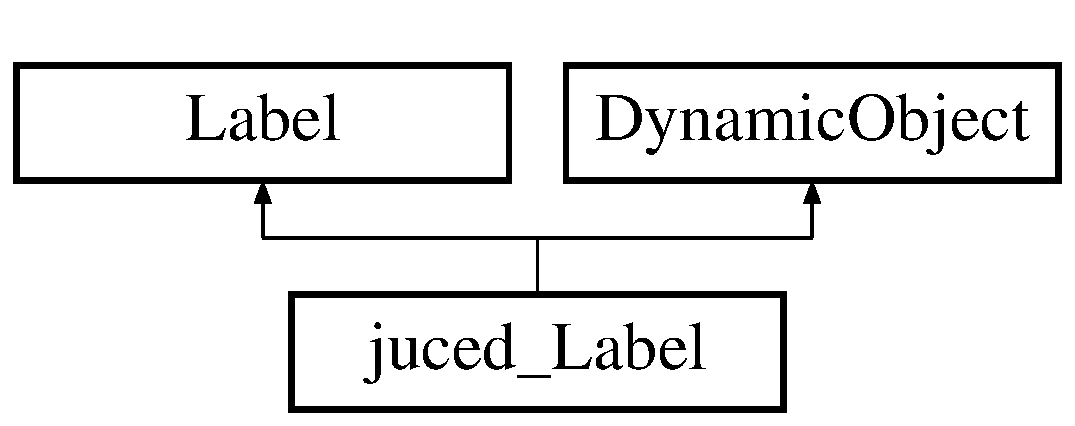
\includegraphics[height=2.000000cm]{classjuced___label}
\end{center}
\end{figure}


The documentation for this class was generated from the following files\-:\begin{DoxyCompactItemize}
\item 
Modules/juced\-\_\-\-Label.\-h\item 
Modules/juced\-\_\-\-Label.\-cpp\end{DoxyCompactItemize}

\hypertarget{classjuced___main_component}{\section{juced\-\_\-\-Main\-Component Class Reference}
\label{classjuced___main_component}\index{juced\-\_\-\-Main\-Component@{juced\-\_\-\-Main\-Component}}
}
Inheritance diagram for juced\-\_\-\-Main\-Component\-:\begin{figure}[H]
\begin{center}
\leavevmode
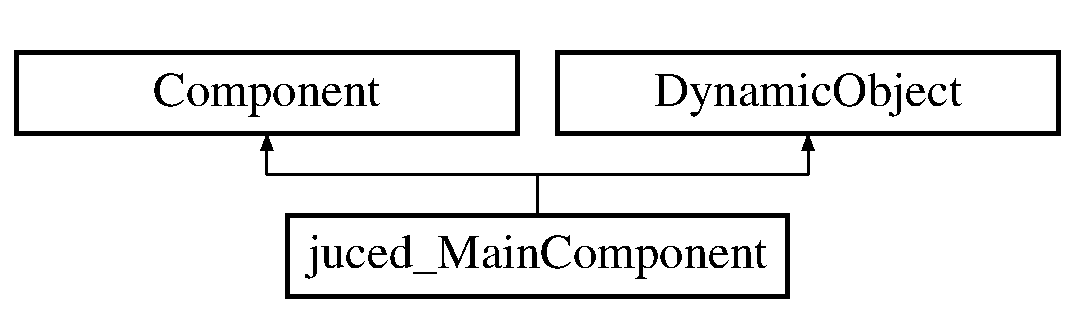
\includegraphics[height=2.000000cm]{classjuced___main_component}
\end{center}
\end{figure}
\subsection*{Public Member Functions}
\begin{DoxyCompactItemize}
\item 
\hypertarget{classjuced___main_component_a1eb5fa768f44c0a13d26d84e04828d6e}{void {\bfseries paint} (Graphics \&)}\label{classjuced___main_component_a1eb5fa768f44c0a13d26d84e04828d6e}

\item 
\hypertarget{classjuced___main_component_aaba6bf2fb0c9ca18a24255336cf74ced}{void {\bfseries resized} ()}\label{classjuced___main_component_aaba6bf2fb0c9ca18a24255336cf74ced}

\end{DoxyCompactItemize}


The documentation for this class was generated from the following files\-:\begin{DoxyCompactItemize}
\item 
Modules/juced\-\_\-\-Main\-Component.\-h\item 
Modules/juced\-\_\-\-Main\-Component.\-cpp\end{DoxyCompactItemize}

\hypertarget{classjuced___text_button}{\section{juced\-\_\-\-Text\-Button Class Reference}
\label{classjuced___text_button}\index{juced\-\_\-\-Text\-Button@{juced\-\_\-\-Text\-Button}}
}
Inheritance diagram for juced\-\_\-\-Text\-Button\-:\begin{figure}[H]
\begin{center}
\leavevmode
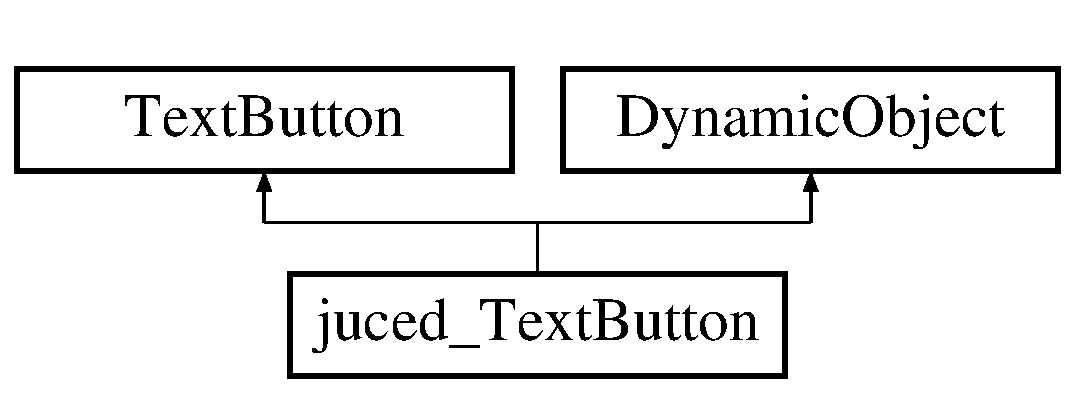
\includegraphics[height=2.000000cm]{classjuced___text_button}
\end{center}
\end{figure}


The documentation for this class was generated from the following files\-:\begin{DoxyCompactItemize}
\item 
Modules/juced\-\_\-\-Text\-Button.\-h\item 
Modules/juced\-\_\-\-Text\-Button.\-cpp\end{DoxyCompactItemize}

\hypertarget{classjuced___window}{\section{juced\-\_\-\-Window Class Reference}
\label{classjuced___window}\index{juced\-\_\-\-Window@{juced\-\_\-\-Window}}
}
Inheritance diagram for juced\-\_\-\-Window\-:\begin{figure}[H]
\begin{center}
\leavevmode
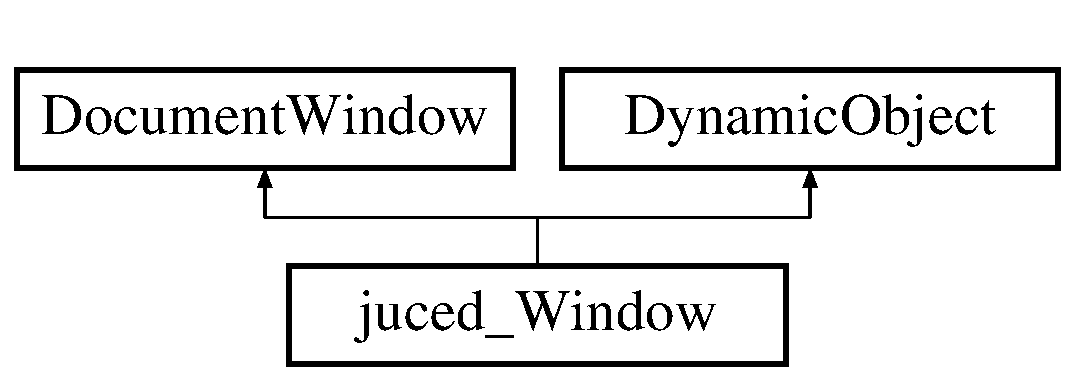
\includegraphics[height=2.000000cm]{classjuced___window}
\end{center}
\end{figure}
\subsection*{Public Member Functions}
\begin{DoxyCompactItemize}
\item 
\hypertarget{classjuced___window_a88ce694f6478b19974660f6a046475e2}{void {\bfseries close\-Button\-Pressed} ()}\label{classjuced___window_a88ce694f6478b19974660f6a046475e2}

\item 
\hypertarget{classjuced___window_a3651c851d5081ab66dbe888caea5411d}{void {\bfseries set\-Content\-Owned} (Component $\ast$new\-Content\-Component, bool resize\-To\-Fit\-When\-Content\-Changes\-Size)}\label{classjuced___window_a3651c851d5081ab66dbe888caea5411d}

\end{DoxyCompactItemize}
\subsection*{Public Attributes}
\begin{DoxyCompactItemize}
\item 
\hypertarget{classjuced___window_af0f4f5da40c9300990dea9fbb5080be2}{int {\bfseries min\-Width}}\label{classjuced___window_af0f4f5da40c9300990dea9fbb5080be2}

\item 
\hypertarget{classjuced___window_a05a4bab2e2400691e432ad2ad2d2a4f2}{int {\bfseries min\-Height}}\label{classjuced___window_a05a4bab2e2400691e432ad2ad2d2a4f2}

\end{DoxyCompactItemize}


The documentation for this class was generated from the following files\-:\begin{DoxyCompactItemize}
\item 
Modules/juced\-\_\-\-Window.\-h\item 
Modules/juced\-\_\-\-Window.\-cpp\end{DoxyCompactItemize}

\hypertarget{classjuced_application}{\section{juced\-Application Class Reference}
\label{classjuced_application}\index{juced\-Application@{juced\-Application}}
}
Inheritance diagram for juced\-Application\-:\begin{figure}[H]
\begin{center}
\leavevmode
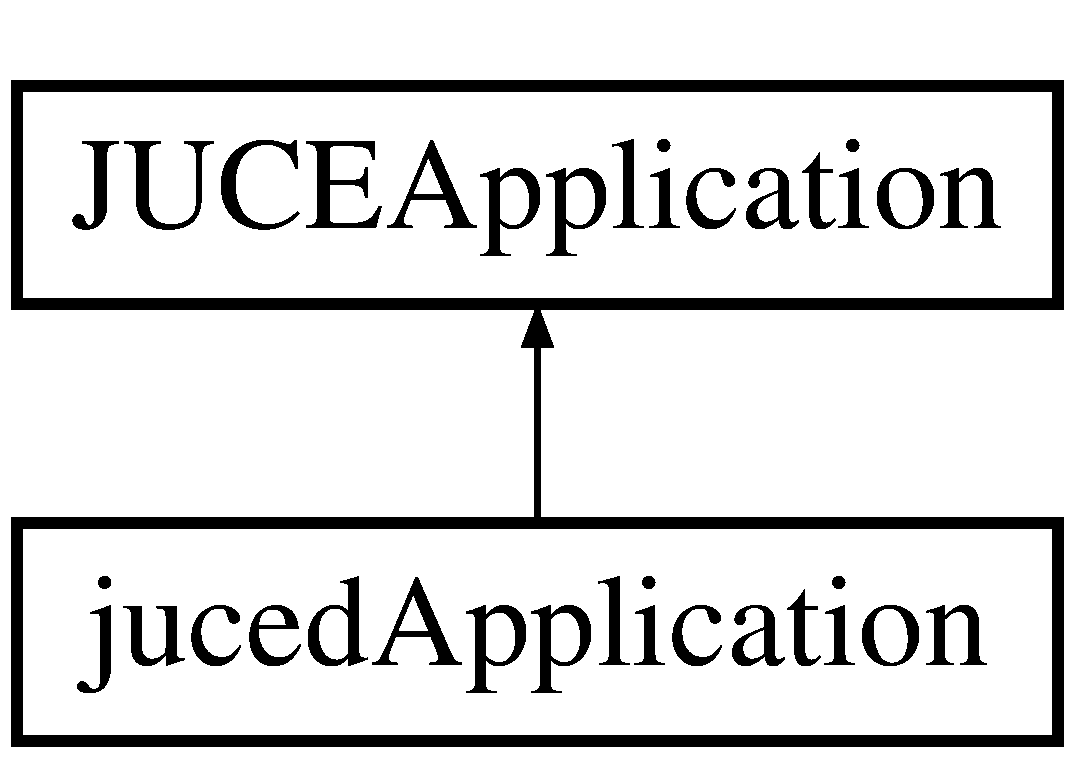
\includegraphics[height=2.000000cm]{classjuced_application}
\end{center}
\end{figure}
\subsection*{Classes}
\begin{DoxyCompactItemize}
\item 
class \hyperlink{classjuced_application_1_1_main_window}{Main\-Window}
\end{DoxyCompactItemize}
\subsection*{Public Member Functions}
\begin{DoxyCompactItemize}
\item 
\hypertarget{classjuced_application_ac8359cc003408393d1c8ffb037fb6100}{const String {\bfseries get\-Application\-Name} ()}\label{classjuced_application_ac8359cc003408393d1c8ffb037fb6100}

\item 
\hypertarget{classjuced_application_a8f9a4e7898e52c2524732e7b383a5410}{const String {\bfseries get\-Application\-Version} ()}\label{classjuced_application_a8f9a4e7898e52c2524732e7b383a5410}

\item 
\hypertarget{classjuced_application_ac4333a950fa796584c2148d79c24759a}{bool {\bfseries more\-Than\-One\-Instance\-Allowed} ()}\label{classjuced_application_ac4333a950fa796584c2148d79c24759a}

\item 
\hypertarget{classjuced_application_ae6fb37901a7ff5cff03dab675b3addbc}{void {\bfseries initialise} (const String \&command\-Line)}\label{classjuced_application_ae6fb37901a7ff5cff03dab675b3addbc}

\item 
\hypertarget{classjuced_application_a0797b147fcec847bd1823841b6c1a537}{void {\bfseries shutdown} ()}\label{classjuced_application_a0797b147fcec847bd1823841b6c1a537}

\item 
\hypertarget{classjuced_application_a54020d2b1ceeb103551c1c6db46a4a93}{void {\bfseries system\-Requested\-Quit} ()}\label{classjuced_application_a54020d2b1ceeb103551c1c6db46a4a93}

\item 
\hypertarget{classjuced_application_a660585773f17554bd062bb9ae2e27358}{void {\bfseries another\-Instance\-Started} (const String \&command\-Line)}\label{classjuced_application_a660585773f17554bd062bb9ae2e27358}

\end{DoxyCompactItemize}


The documentation for this class was generated from the following file\-:\begin{DoxyCompactItemize}
\item 
Main.\-cpp\end{DoxyCompactItemize}

\hypertarget{class_main_content_component}{\section{Main\-Content\-Component Class Reference}
\label{class_main_content_component}\index{Main\-Content\-Component@{Main\-Content\-Component}}
}
Inheritance diagram for Main\-Content\-Component\-:\begin{figure}[H]
\begin{center}
\leavevmode
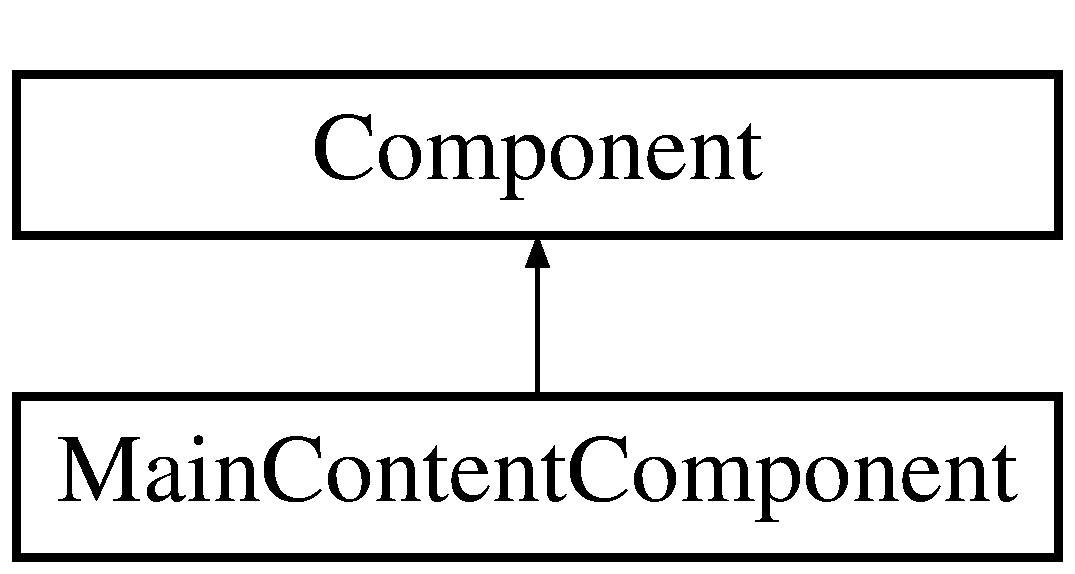
\includegraphics[height=2.000000cm]{class_main_content_component}
\end{center}
\end{figure}
\subsection*{Public Member Functions}
\begin{DoxyCompactItemize}
\item 
\hypertarget{class_main_content_component_a897ff27920dedae2b120fe4e6a198815}{void {\bfseries paint} (Graphics \&)}\label{class_main_content_component_a897ff27920dedae2b120fe4e6a198815}

\item 
\hypertarget{class_main_content_component_a42ef2312ea53596306779503fdce5992}{void {\bfseries resized} ()}\label{class_main_content_component_a42ef2312ea53596306779503fdce5992}

\end{DoxyCompactItemize}


The documentation for this class was generated from the following files\-:\begin{DoxyCompactItemize}
\item 
Main\-Component.\-h\item 
Main\-Component.\-cpp\end{DoxyCompactItemize}

\hypertarget{classjuced_application_1_1_main_window}{\section{juced\-Application\-:\-:Main\-Window Class Reference}
\label{classjuced_application_1_1_main_window}\index{juced\-Application\-::\-Main\-Window@{juced\-Application\-::\-Main\-Window}}
}
Inheritance diagram for juced\-Application\-:\-:Main\-Window\-:\begin{figure}[H]
\begin{center}
\leavevmode
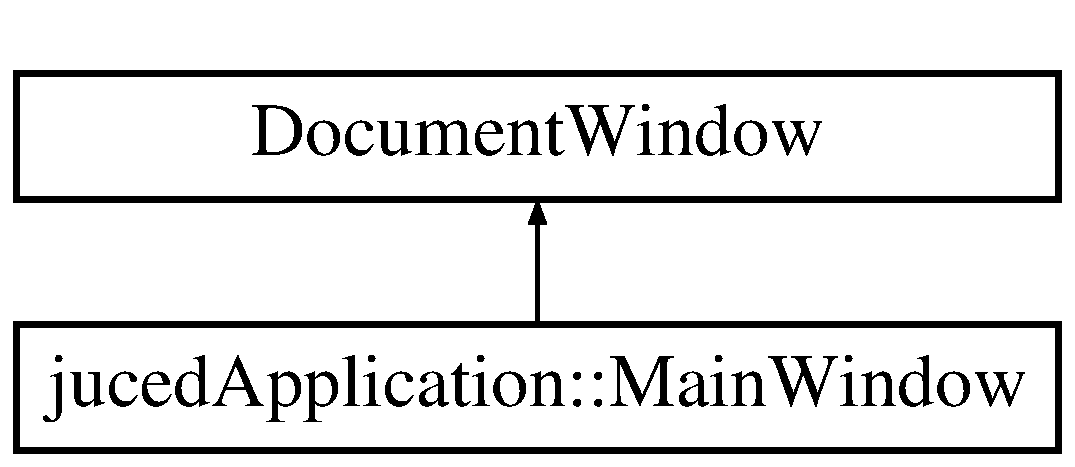
\includegraphics[height=2.000000cm]{classjuced_application_1_1_main_window}
\end{center}
\end{figure}
\subsection*{Public Member Functions}
\begin{DoxyCompactItemize}
\item 
\hypertarget{classjuced_application_1_1_main_window_aeeb894e5b022565b67601273d978d4cb}{void {\bfseries close\-Button\-Pressed} ()}\label{classjuced_application_1_1_main_window_aeeb894e5b022565b67601273d978d4cb}

\end{DoxyCompactItemize}


The documentation for this class was generated from the following file\-:\begin{DoxyCompactItemize}
\item 
Main.\-cpp\end{DoxyCompactItemize}

\hypertarget{class_property_group}{\section{Property\-Group Class Reference}
\label{class_property_group}\index{Property\-Group@{Property\-Group}}
}
Inheritance diagram for Property\-Group\-:\begin{figure}[H]
\begin{center}
\leavevmode
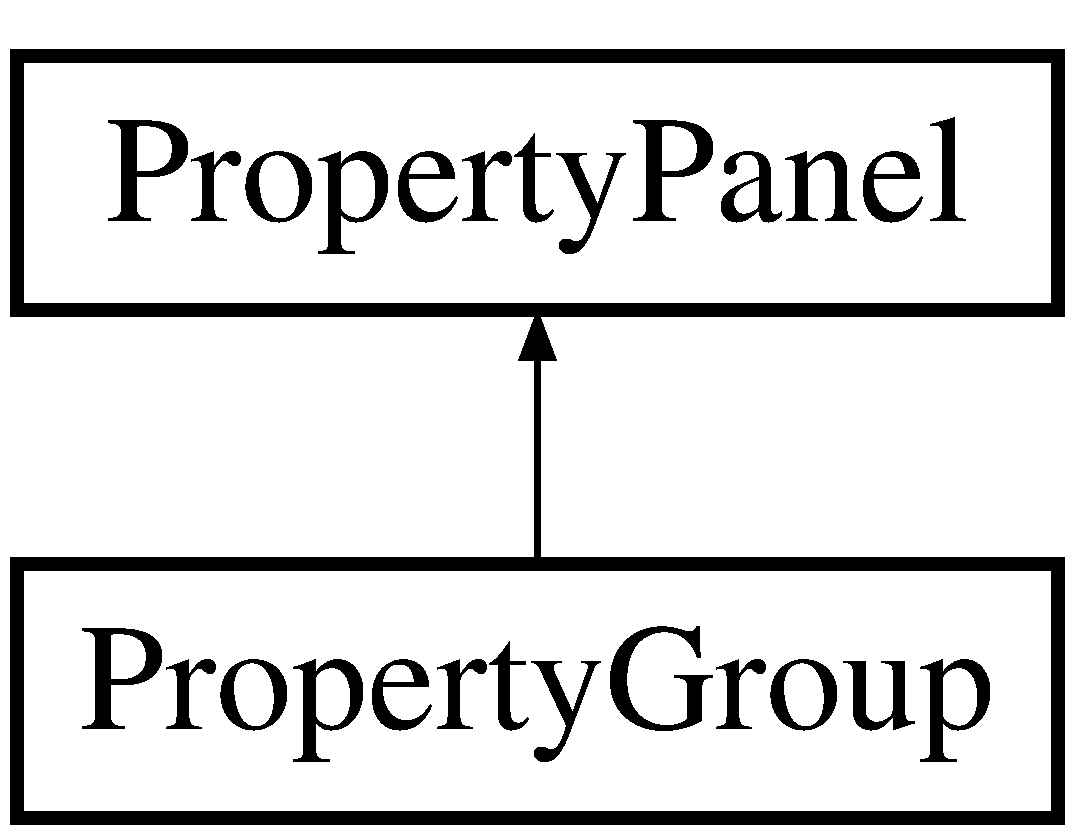
\includegraphics[height=2.000000cm]{class_property_group}
\end{center}
\end{figure}
\subsection*{Public Member Functions}
\begin{DoxyCompactItemize}
\item 
\hypertarget{class_property_group_a100e95cb8e880c2c622c0b77d1f1afe5}{{\bfseries Property\-Group} (Value\-Tree $\ast$tree)}\label{class_property_group_a100e95cb8e880c2c622c0b77d1f1afe5}

\end{DoxyCompactItemize}


The documentation for this class was generated from the following file\-:\begin{DoxyCompactItemize}
\item 
Designer/Properties\-Component.\-cpp\end{DoxyCompactItemize}

\hypertarget{class_property_view}{\section{Property\-View Class Reference}
\label{class_property_view}\index{Property\-View@{Property\-View}}
}
Inheritance diagram for Property\-View\-:\begin{figure}[H]
\begin{center}
\leavevmode
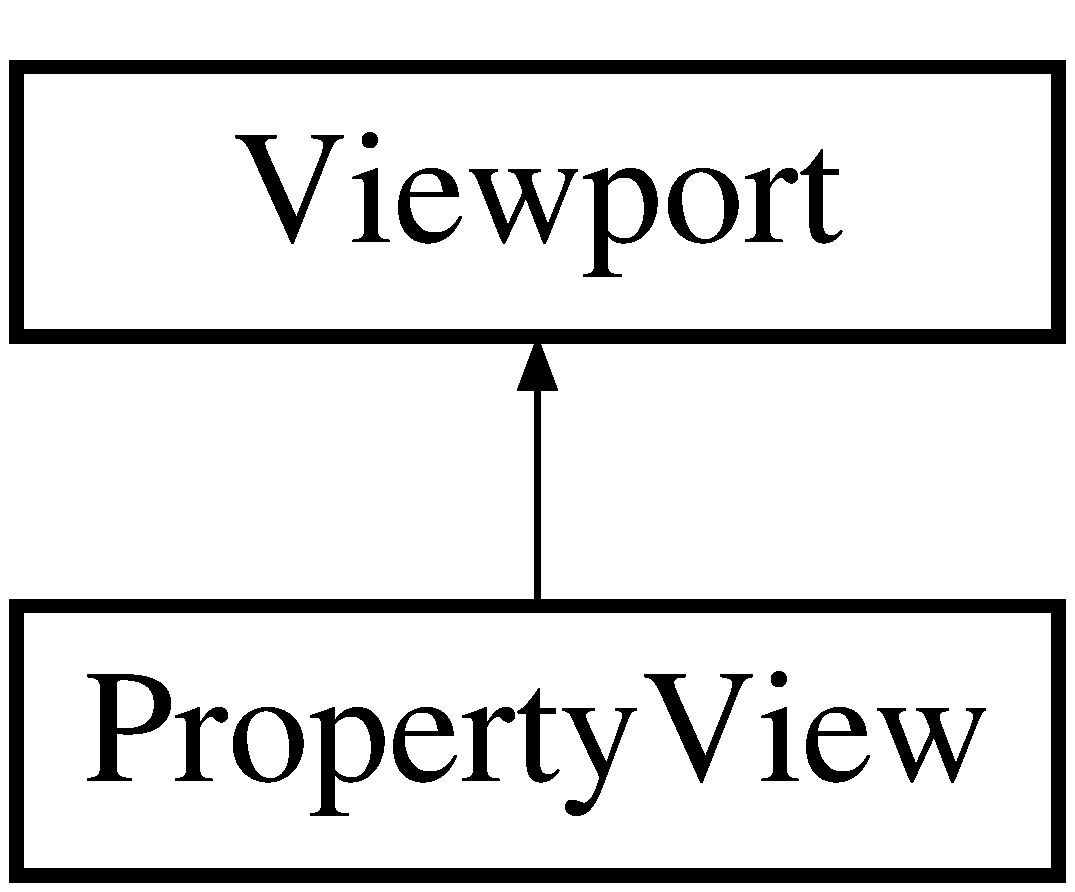
\includegraphics[height=2.000000cm]{class_property_view}
\end{center}
\end{figure}
\subsection*{Public Member Functions}
\begin{DoxyCompactItemize}
\item 
\hypertarget{class_property_view_af0d12aebca62216edcedcff29e83cf74}{{\bfseries Property\-View} (Component $\ast$content)}\label{class_property_view_af0d12aebca62216edcedcff29e83cf74}

\item 
\hypertarget{class_property_view_a91a0862621a5f073b4e280bd3d1286ba}{void {\bfseries set\-Viewed\-Component} (Component $\ast$content)}\label{class_property_view_a91a0862621a5f073b4e280bd3d1286ba}

\item 
\hypertarget{class_property_view_a51c887a8a5c32b0c6dc6f42c23576c06}{void {\bfseries paint} (Graphics \&g)}\label{class_property_view_a51c887a8a5c32b0c6dc6f42c23576c06}

\item 
\hypertarget{class_property_view_aa59022f09d173dbe026187e243768207}{void {\bfseries resized} ()}\label{class_property_view_aa59022f09d173dbe026187e243768207}

\end{DoxyCompactItemize}


The documentation for this class was generated from the following file\-:\begin{DoxyCompactItemize}
\item 
Designer/Properties\-Component.\-cpp\end{DoxyCompactItemize}

\hypertarget{class_selection_area}{\section{Selection\-Area Class Reference}
\label{class_selection_area}\index{Selection\-Area@{Selection\-Area}}
}
Inheritance diagram for Selection\-Area\-:\begin{figure}[H]
\begin{center}
\leavevmode
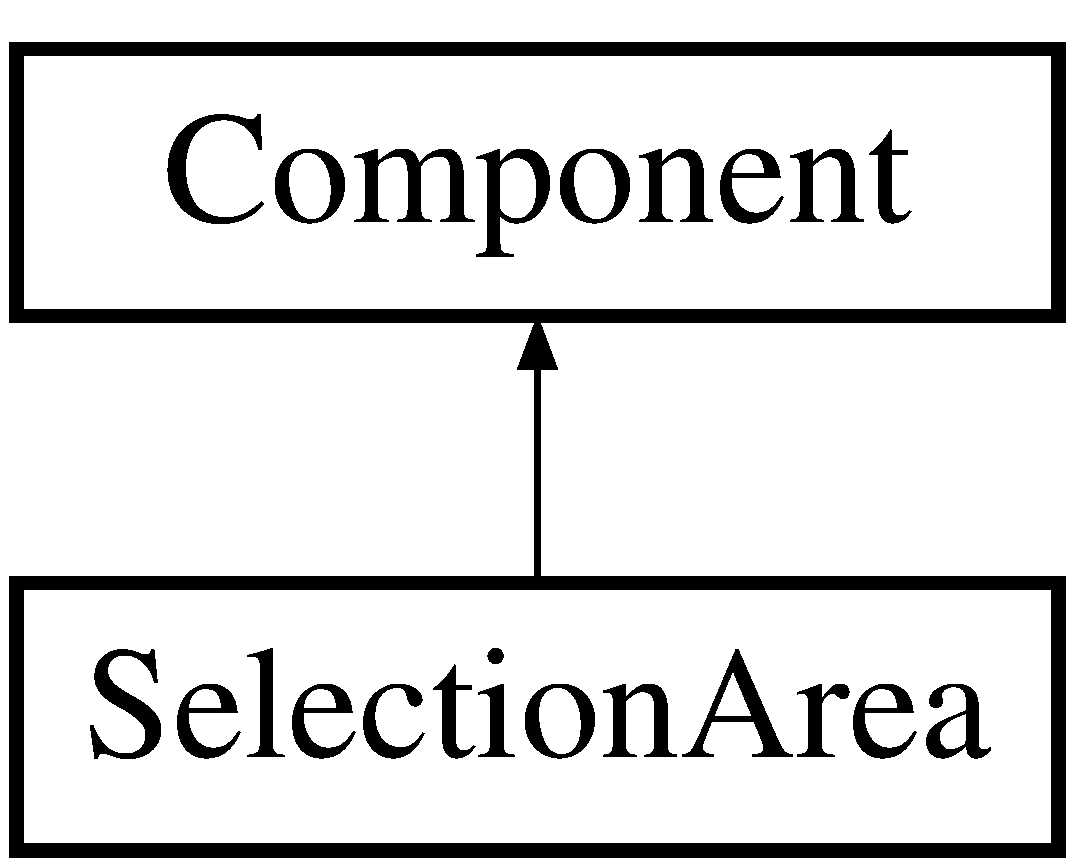
\includegraphics[height=2.000000cm]{class_selection_area}
\end{center}
\end{figure}
\subsection*{Public Member Functions}
\begin{DoxyCompactItemize}
\item 
\hypertarget{class_selection_area_a8969a10e71d1675dd00de1015d9e1580}{{\bfseries Selection\-Area} (bool \-\_\-is\-Component\-Selection)}\label{class_selection_area_a8969a10e71d1675dd00de1015d9e1580}

\item 
\hypertarget{class_selection_area_aeede81851c600f718effb036859c448f}{void {\bfseries set\-Selection\-Bounds} (int x, int y, int width, int height)}\label{class_selection_area_aeede81851c600f718effb036859c448f}

\item 
\hypertarget{class_selection_area_ad6c2bd41ddd45e4e5a114c445664cb0e}{void {\bfseries set\-Visible} (bool should\-Be\-Visible)}\label{class_selection_area_ad6c2bd41ddd45e4e5a114c445664cb0e}

\item 
\hypertarget{class_selection_area_afb580cfc63418ee93ecf06bc3ae3dffe}{bool {\bfseries is\-Ready} ()}\label{class_selection_area_afb580cfc63418ee93ecf06bc3ae3dffe}

\item 
\hypertarget{class_selection_area_a7028c04b01c5c229510492e8d71399ea}{void {\bfseries paint} (Graphics \&g)}\label{class_selection_area_a7028c04b01c5c229510492e8d71399ea}

\item 
\hypertarget{class_selection_area_ae043b740d095421016b6b7e9bc2e8a64}{void {\bfseries mouse\-Drag} (const Mouse\-Event \&event)}\label{class_selection_area_ae043b740d095421016b6b7e9bc2e8a64}

\item 
\hypertarget{class_selection_area_aa25f2e2d5c4d54eedbb5567b4dcc9faf}{void {\bfseries set\-Box\-Size} (int new\-Size)}\label{class_selection_area_aa25f2e2d5c4d54eedbb5567b4dcc9faf}

\item 
\hypertarget{class_selection_area_acb552e98fe92a11f205f0c14eac69032}{int {\bfseries get\-Box\-Size} ()}\label{class_selection_area_acb552e98fe92a11f205f0c14eac69032}

\end{DoxyCompactItemize}


The documentation for this class was generated from the following file\-:\begin{DoxyCompactItemize}
\item 
Designer/Selection\-Area.\-cpp\end{DoxyCompactItemize}

\hypertarget{class_text_with_button_property_component}{\section{Text\-With\-Button\-Property\-Component Class Reference}
\label{class_text_with_button_property_component}\index{Text\-With\-Button\-Property\-Component@{Text\-With\-Button\-Property\-Component}}
}
Inheritance diagram for Text\-With\-Button\-Property\-Component\-:\begin{figure}[H]
\begin{center}
\leavevmode
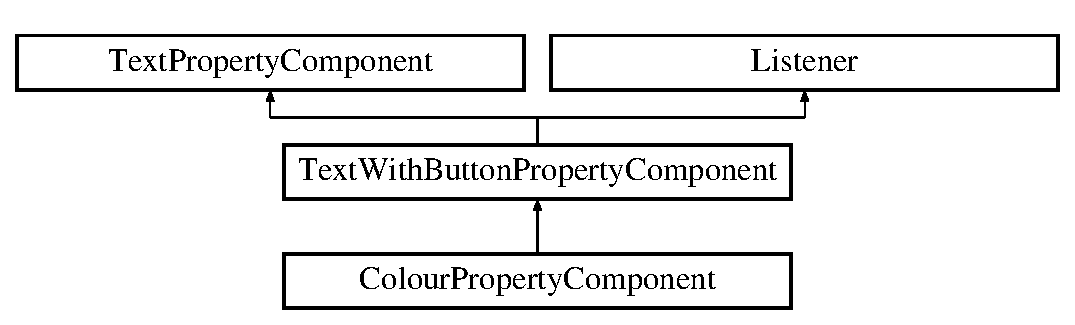
\includegraphics[height=3.000000cm]{class_text_with_button_property_component}
\end{center}
\end{figure}
\subsection*{Public Member Functions}
\begin{DoxyCompactItemize}
\item 
\hypertarget{class_text_with_button_property_component_a6e0602af61cefd723f2de39afc30bbdd}{{\bfseries Text\-With\-Button\-Property\-Component} (const Value \&Value\-To\-Control, const String \&property\-Name)}\label{class_text_with_button_property_component_a6e0602af61cefd723f2de39afc30bbdd}

\item 
\hypertarget{class_text_with_button_property_component_a8c9ffa8ad1454bff3af84d58133b7c0c}{void {\bfseries resized} ()}\label{class_text_with_button_property_component_a8c9ffa8ad1454bff3af84d58133b7c0c}

\end{DoxyCompactItemize}
\subsection*{Public Attributes}
\begin{DoxyCompactItemize}
\item 
\hypertarget{class_text_with_button_property_component_a82ee855aed4a255728c610dda7f7821b}{Text\-Button $\ast$ {\bfseries button}}\label{class_text_with_button_property_component_a82ee855aed4a255728c610dda7f7821b}

\item 
\hypertarget{class_text_with_button_property_component_a55480a356c71b7ed5b81fcbf0e390a68}{Label $\ast$ {\bfseries text\-Label}}\label{class_text_with_button_property_component_a55480a356c71b7ed5b81fcbf0e390a68}

\end{DoxyCompactItemize}


The documentation for this class was generated from the following file\-:\begin{DoxyCompactItemize}
\item 
Designer/Properties\-Component.\-cpp\end{DoxyCompactItemize}

\hypertarget{class_toolbox}{\section{Toolbox Class Reference}
\label{class_toolbox}\index{Toolbox@{Toolbox}}
}
Inheritance diagram for Toolbox\-:\begin{figure}[H]
\begin{center}
\leavevmode
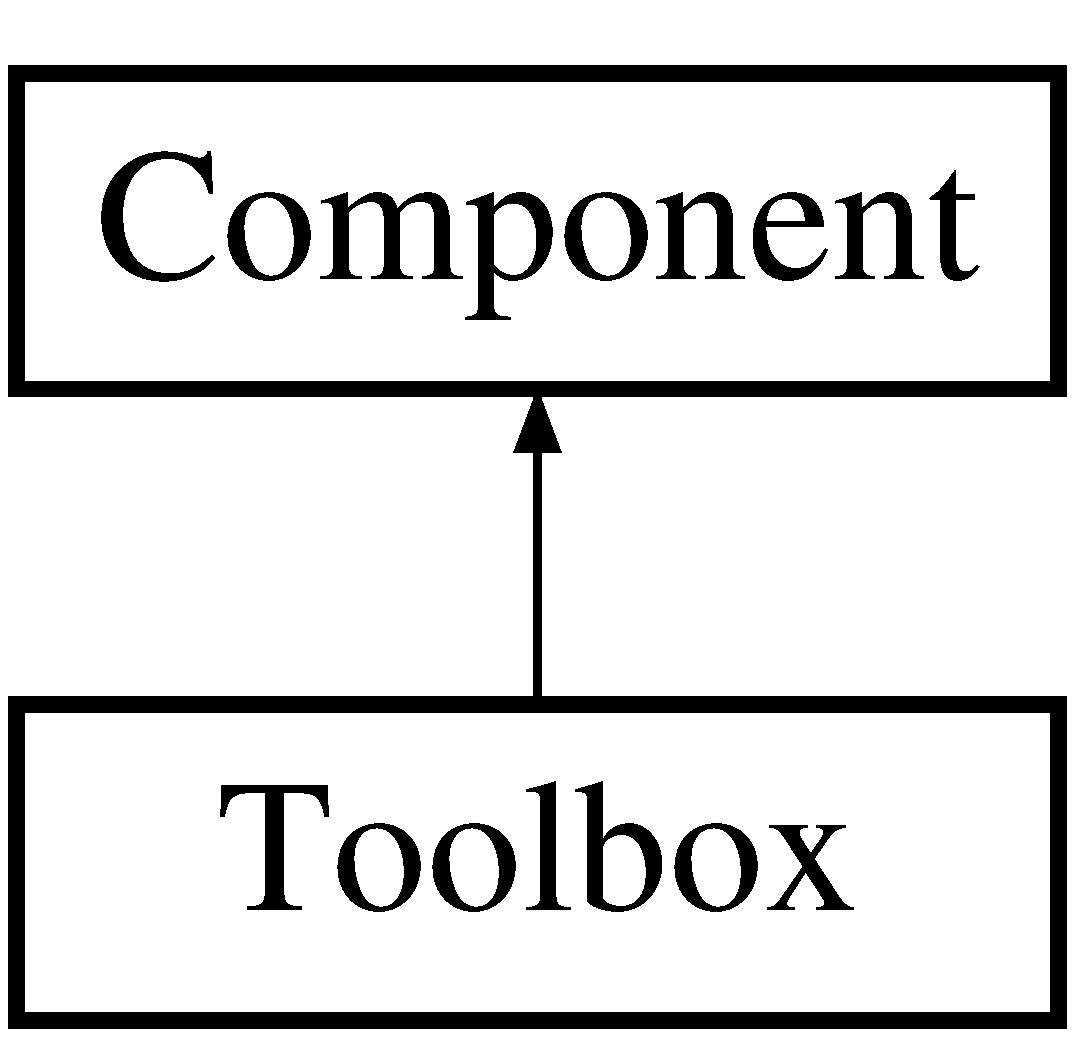
\includegraphics[height=2.000000cm]{class_toolbox}
\end{center}
\end{figure}
\subsection*{Public Member Functions}
\begin{DoxyCompactItemize}
\item 
\hypertarget{class_toolbox_a70c729ee9d13e2006dde37d6d3799b5e}{{\bfseries Toolbox} (int \-\_\-items\-Per\-Row, int \-\_\-item\-Size, int \-\_\-item\-Padding)}\label{class_toolbox_a70c729ee9d13e2006dde37d6d3799b5e}

\item 
\hypertarget{class_toolbox_a4670a8e31d3351f9cffdef9afab55f60}{void {\bfseries set\-Bounds} (int x, int y, int width, int height)}\label{class_toolbox_a4670a8e31d3351f9cffdef9afab55f60}

\item 
\hypertarget{class_toolbox_a30371096bc1cd84effacb0e1fb5f7118}{void {\bfseries load\-Tooltips} ()}\label{class_toolbox_a30371096bc1cd84effacb0e1fb5f7118}

\item 
\hypertarget{class_toolbox_a132ff7cc3572441f2d1d79ae92b13d7c}{void {\bfseries add\-Item} (const String \&name, const String \&tool\-Tip, const char $\ast$image, int image\-Size)}\label{class_toolbox_a132ff7cc3572441f2d1d79ae92b13d7c}

\item 
\hypertarget{class_toolbox_a944da05e258adeae77b7ca4e3a45c346}{void {\bfseries paint} (Graphics \&g)}\label{class_toolbox_a944da05e258adeae77b7ca4e3a45c346}

\item 
\hypertarget{class_toolbox_a7a983d8c084a6ba37039cbcce4d4248e}{String $\ast$ {\bfseries get\-Selected\-Tool\-Name} ()}\label{class_toolbox_a7a983d8c084a6ba37039cbcce4d4248e}

\item 
\hypertarget{class_toolbox_a65107fbc493085353192613880d66b5e}{void {\bfseries deselect\-Tool} ()}\label{class_toolbox_a65107fbc493085353192613880d66b5e}

\item 
\hypertarget{class_toolbox_a3fb98eec070a42902f04bce8071f7588}{void {\bfseries mouse\-Up} (const Mouse\-Event \&event)}\label{class_toolbox_a3fb98eec070a42902f04bce8071f7588}

\end{DoxyCompactItemize}


The documentation for this class was generated from the following file\-:\begin{DoxyCompactItemize}
\item 
Designer/Toolbox.\-cpp\end{DoxyCompactItemize}

\addcontentsline{toc}{part}{Index}
\printindex
\end{document}
